% arara: xelatex
% arara: xelatex
% arara: xelatex

% options:
% thesis=B bachelor's thesis
% thesis=M master's thesis
% czech thesis in Czech language
% english thesis in English language
% hidelinks remove color boxes around hyperlinks

\documentclass[thesis=M,english]{FITthesis}[2012/10/20]

\usepackage{graphicx} %graphics files inclusion
% \usepackage{subfig} %subfigures
% \usepackage{amsmath} %advanced maths
% \usepackage{amssymb} %additional math symbols

\usepackage{dirtree} %directory tree visualisation

% list of acronyms
% \usepackage[acronym,nonumberlist,toc,numberedsection=autolabel,nomain]{glossaries}
\iflanguage{czech}{\renewcommand*{\acronymname}{Seznam pou{\v z}it{\' y}ch zkratek}}{}
% \makeglossaries

\newcommand{\tg}{\mathop{\mathrm{tg}}} %cesky tangens
\newcommand{\cotg}{\mathop{\mathrm{cotg}}} %cesky cotangens

% % % % % % % % % % % % % % % % % % % % % % % % % % % % % % % % % % % 
% % % % % % % % % % % % % % % % % % % % % % % % % % % % % % % % % % % 
\department{Department of Applied Mathematics}
\title{Detecting similarities of data domains using machine learning methods}
\authorGN{Andrej Oliver} 
\authorFN{Chud\'y}
\authorWithDegrees{Bc. Andrej Oliver Chud\'y} 
\author{Andrej Oliver Chud\'y} 
\supervisor{Ing. Zdenek Buk, Ph.D.}
\acknowledgements{I would like to thank my family and friends for support during writing this thesis.}
\abstractCS{
% TODO abstractCS
}
\abstractEN{
% TODO abstractEN
}
\placeForDeclarationOfAuthenticity{Prague} 
\keywordsCS{
% TODO KeywordsCCS
}
\keywordsEN{Natural Language Processing, Deep learning, NLP, RNN, CNN, embedding, LSTM, GRU.}
\declarationOfAuthenticityOption{4} %select as appropriate, according to the desired license
\website{http://site.example/thesis} %optional URL (remove entirely if you have no URL for this thesis)

\begin{document}


\begin{introduction}

	\section{Objectives}

	\section{Challenges}

\end{introduction}

\chapter{Preliminaries}

\section{What is Deep Learning?}
First, we need to define clearly what we're talking about. What deep learning is? Deep learning is a specific subfield of machine learning. The deep in deep learning isn't a reference to any kind of deeper understanding but it stands for the idea of successive layers of representations. The count of layers contribute to a model called the depth of the model. Modern deep learning often involves tens or even hundreds of successive layers of representations and they've all learned automatically from exposure training data. In deep learning, these layered representations are (almost always) learned via models called neural networks, structured in literal layers stacked on top of each other. On the next image, you can see how a network several layers deep look like. \cite{DLwP}


\begin{figure}\centering
	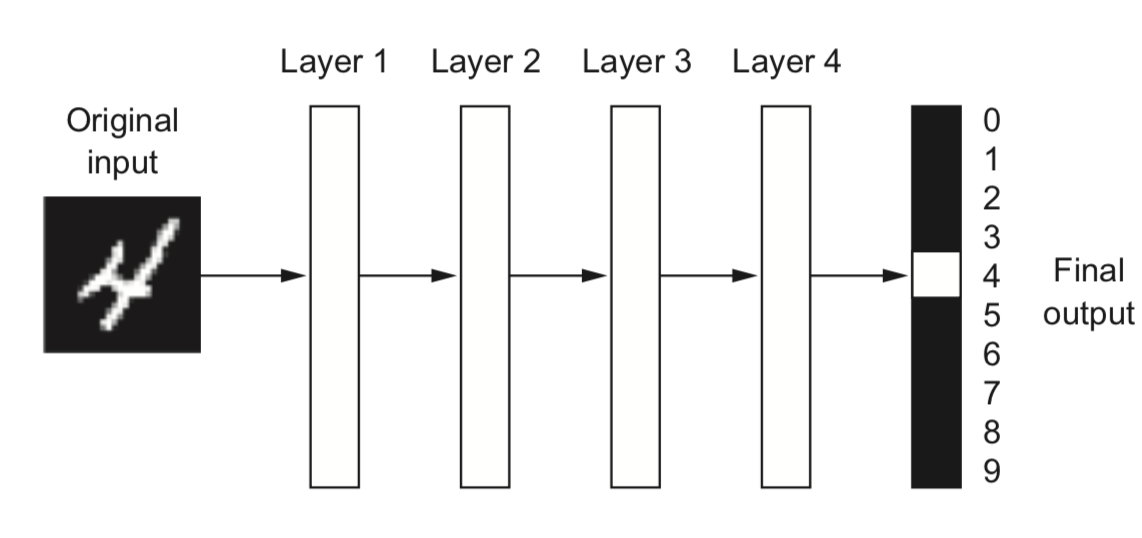
\includegraphics[scale=0.6]{images/deep_NN}
	\caption{Deep neural network}\label{fig:deep NN}
\end{figure}

\subsection{Training of neural networks}
The learning process in a neural network is about mapping inputs (image, text, or something else) to target (some label such as category or continues value) via a deep sequence of simple transformations (layers) and that these data transformations are learned by exposure to examples. 

The specification of what a layer does to its input data is stored in the layer's weights, which in essence are a bunch of numbers. In technical terms, we'd say that the transformation implemented by a layer is parameterized by its weights. In this context, learning means finding a set of values for the weights of all layers in a network, such that the network will correctly map example inputs to their associated targets. But a deep neural network can contain tens of millions of parameters. Finding the correct values for all of them is a very hard optimization task. 

To judge the output of a neural network, you need to be able to measure how far this output is from what you expected. This is the job of the \textbf{loss function} of the network. The \textbf{loss function} takes the predictions of the network and the true target and computes a distance score, capturing how well the network has done on this specific example. The fundamental trick in deep learning is to use this score as a feedback signal to adjust the value of the weights a little, in a direction that will lower the loss score for the current example. This adjustment is the job of the \textbf{optimizer}, which implements what's called the \textbf{Backpropagation} algorithm which is the most famous algorithm in machine learning for optimization of hyperparametric space of NN. \nocite{DLwP}

\subsection{Loss functions}
The loss function is the bread and butter of modern machine learning. It's very easy. It's a method of evaluating how good a model solving the problem over specific take data. Loss functions can be categorized into two types:
\begin{itemize}
  \item \textbf{Classification loss} (SVMLoss, Cross Entropy and more) 
  \item \textbf{Regression loss} (MSE, MAE, MBE and more)
\end{itemize}



\subsection{Optimizetor}
% TODO optimizers



\section{Recurrent neural networks}
A principal of the work of the recurrent neural network is more similar to the human brain. Biological intelligence processes information incrementally. Built from past information and constantly updated as new information comes in. Traditional feed-forward neural networks can't do this. Recurrent neural network (RNN) address this problem. Those networks contain loops, allowing persist information the other words RNN has memory. This allows it to exhibit temporal dynamic behavior. Historically, these networks have been difficult to train, but more recently, advances in research (optimization, network architectures, parallelism, and graphics processing units [GPUs]) have made them more approachable for the practitioner. RNNs have a huge success in speech recognition, language modeling, translation, image captioning and more.


\begin{figure}\centering
	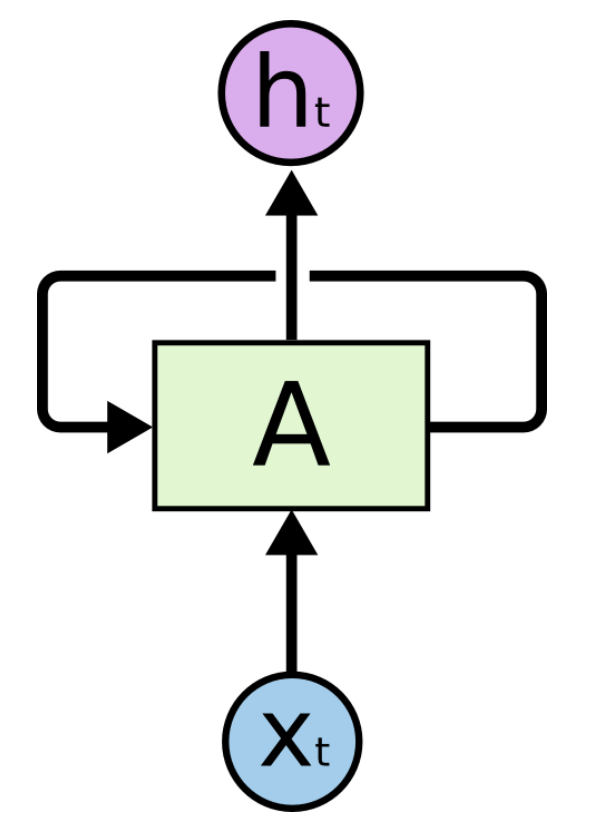
\includegraphics[scale=0.5]{images/RNN_diagram}
	\caption{RNN  with loop}\label{fig:RNN_loop}
\end{figure}

RNNs are considered Turing complete and well suited for problems witch the input and/or output is composed of vectors that involve a time dependency between the values. It processes sequences by iterating through the sequence elements and maintaining a state (see figure \ref{fig:RNN_loop}). 

 
\subsection{Long Short Term Memory (LSTM)}
It is a special kind of RNN, capable of learning long-term dependences. LSTMs are explicitly designed to avoid the long-term dependency problem. Remembering information for long periods of time is practically their default behavior, not something they struggle to learn!



\begin{figure}\centering
	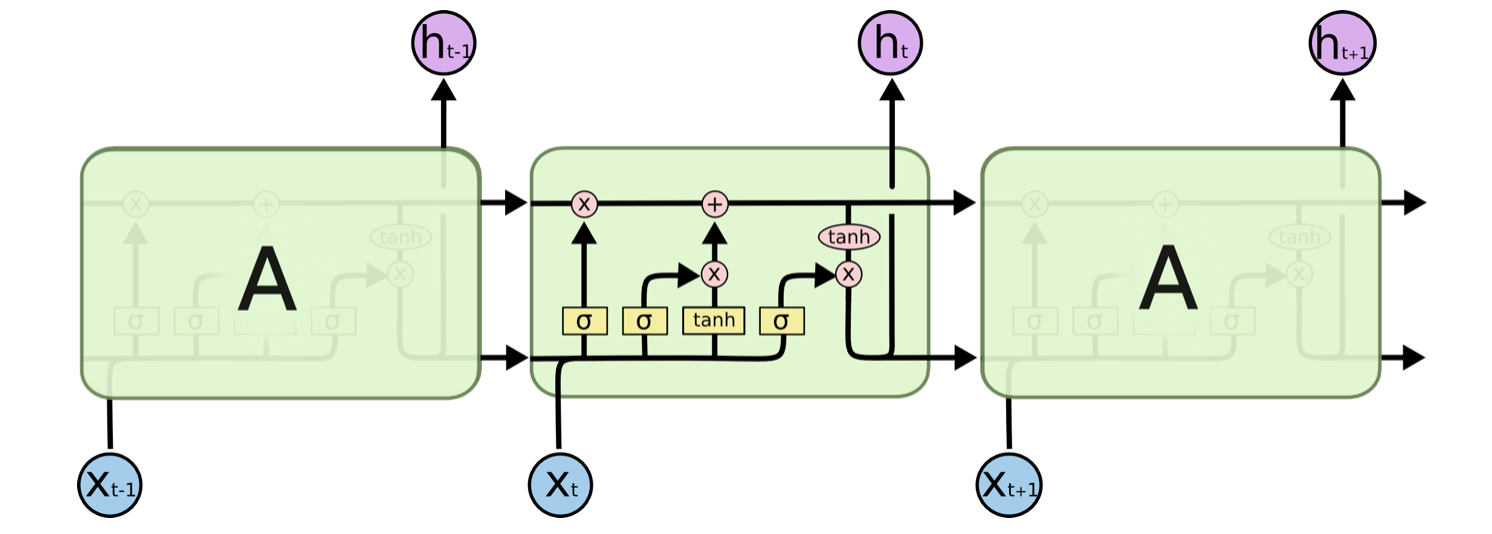
\includegraphics[scale=0.5]{images/LSTM_1}
	\caption{Repeating module in an LSTM contains four interacting layers.}\label{fig:LSTM}
\end{figure}

LSTMs are visualizing as the chain with modules, which contains four layers,  interacting in a very special way.





% TODO Convolution neural networks
\section{Summary}



\begin{conclusion}

\end{conclusion}

\bibliographystyle{iso690.bst}
\bibliography{ref}

\appendix

% \printglossaries

\chapter{Contents of CD}\label{app:CDcontent}


\begin{figure}
	\dirtree{%
		.1 readme.txt\DTcomment{the file with CD contents description}.
		.1 data\DTcomment{the data files directory}.
		.2 graphs\DTcomment{the directory of graphs of experiments}.
		.3 *.eps\DTcomment{the B/W graphs}.
		.3 *.png\DTcomment{the color graphs}.
		.3 *.dat\DTcomment{the graphs data files}.
		.1 exe\DTcomment{the directory with executable WBDCM program}.
		.2 wbdcm\DTcomment{the WBDCM program executable (UNIX)}.
		.2 wbdcm.exe\DTcomment{the WBDCM program executable (Windows)}.
		.1 src\DTcomment{the directory of source codes}.
		.2 wbdcm\DTcomment{the directory of WBDCM program}.
		.3 Makefile\DTcomment{the makefile of WBDCM program (UNIX)}.
		.2 thesis\DTcomment{the directory of \LaTeX{} source codes of the thesis}.
		.3 figures\DTcomment{the thesis figures directory}.
		.3 *.tex\DTcomment{the \LaTeX{} source code files of the thesis}.
		.1 text\DTcomment{the thesis text directory}.
		.2 thesis.pdf\DTcomment{the Diploma thesis in PDF format}.
		.2 thesis.ps\DTcomment{the Diploma thesis in PS format}.
	}
\end{figure}


\end{document}
